\documentclass[journal]{IEEEtran}

% include a few useful packages; you will probably want more
\usepackage{graphicx} 
\usepackage[margin=1in]{geometry} 
\usepackage{amsmath,amsthm,amssymb}
\usepackage[noend]{algpseudocode}
\usepackage[hypcap=true]{caption}
\usepackage{lipsum}
\usepackage{float}
\usepackage{tabularx}
\usepackage{xcolor}
\makeatletter
\def\BState{\State\hskip-\ALG@thistlm}
\makeatother
\usepackage{algorithm}
% place all photos and diagrams in the media folder
\graphicspath{{media/}}

\hyphenation{op-tical net-works semi-conduc-tor}

\begin{document}

\title{%
  Team 11 ROB 550 BotLab Report \\
  %\large Prototype Implementations of SLAM and A* for a Wheeled Robot
  }
    
\author{Yifan Xu,
Varun Aggarwal, Daksh Narang, and Xiaoyu Sun}

\maketitle

\begin{abstract}
In this project, we developed a fully autonomous nonholonomic differential drive robot. We implemented a combination of feedforward and feedback control to control the motions of our robot. Additionally, we implemented a Simultaneous Localization and Mapping (SLAM) algorithm to perceive and process our robot's environment. Furthermore, we implemented A* search algorithm for planning paths in known environments. At large, the project encapsulates action, perception, and reasoning for a ground robot. As a result, our robot can successfully explore an unknown environment autonomously.

\end{abstract}

\IEEEpeerreviewmaketitle

\section{Introduction}
\IEEEPARstart{I}{n} the first part, we want to be able to control the robot's motions manually. In order to accomplish this, we leveraged data from encoders to control the speed of the wheels using our control mechanism. After we are able to control the robot, we move to build a more sophisticated algorithm for mapping and localizing the environment. We first constructed an occupancy grid using known poses. Following that, we implemented Monte Carlo Localization in a known map. Finally, putting together the mapping and localization parts, we created a full SLAM system. With the knowledge of where the robot is and what is in its environment, we implemented planning with A* and a frontier exploration algorithm.

\section{Methodology and Result}
\subsection{Motion and Odometry}
\subsubsection{Wheel Speed Characterization for an Open Loop Controller} \hfill \\

In Classical Control Theory, an open loop approach to control a plant, in this case the left and right motors of our robot, is implemented through a mapping function that takes a setpoint as an input and maps it to the an appropriate controller output (i.e., the signal commanding the actuator). In contrast to the closed loop control approach that monitors and reduces the error, the open loop approach does not minimize the error between the actual and the desired outputs. However, this comes with the drawback of not having a criterion to determine how the actual output compares to the desired output. In this section, we conducted experiments to collect data that helped understand the mathematical relationship between the target setpoint and the motor input signal: open-loop calibration.

We ran each motor from 0.0 m/s up to its maximum possible speed under full load conditions by varying the amount of voltage applied to the motor by varying the duty cycle (Pulse Width Modulation, PWM) of the actuation signal. Through our tests, we collected data from the encoders and processed it to estimate the actual speed the motor spinned at. Based on our data, we fitted an affine mapping function to acquire the mathematical relationship between the two variables.


\begin{figure}[h]
\begin{center}
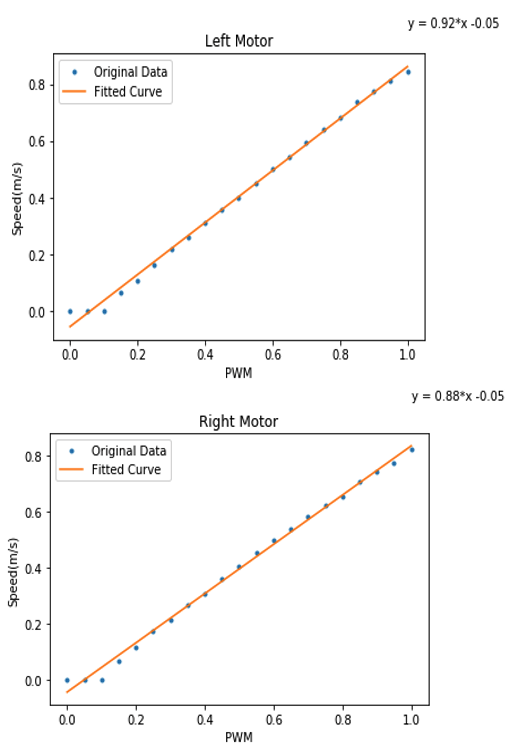
\includegraphics[width=0.9\linewidth]{image_1/figure_1_1_1.jpg}
\end{center}
   \caption{Motor Calibration}
   \label{Figure_1_1_1}
\end{figure}

As can be seen in the graphs in Figure \ref{Figure_1_1_1}, for our teams’ robot, the mathematical relationship between the setpoint and the controller signal is mostly linear except at the starting and ending intervals.\\

\subsubsection{Open and Closed Loop Wheel Speed Controllers} \hfill

\begin{figure*}[h]
\begin{center}
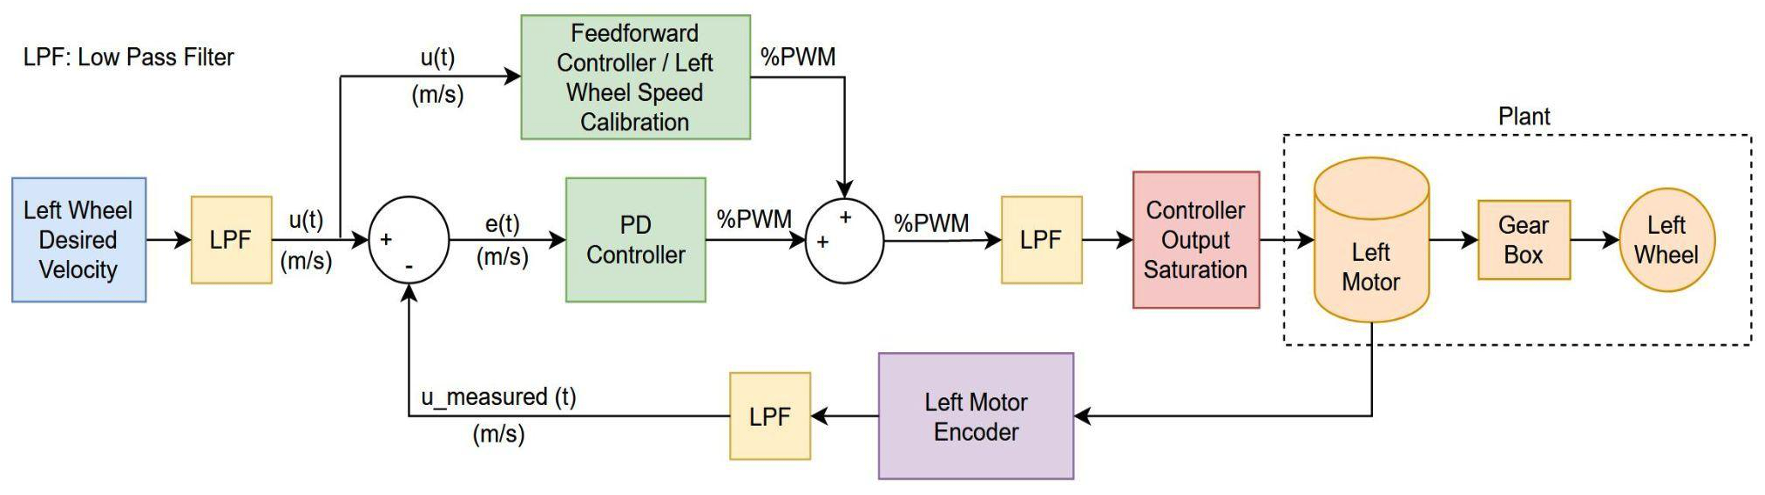
\includegraphics[width=0.83\textwidth]{image_1/figure_1_2_1.jpg}
\end{center}
   \caption{Left wheel’s speed controller’s architecture, right wheel’s speed controller is identical}
   \label{Figure_1_2_1}
\end{figure*}


In order to control the speeds of the left and right wheels of our robot, we implemented a combination of feedforward (FF) and feedback (FB) control mechanisms. The idea behind using FF control was to get the motor running close to the desired or commanded speed. Once the motor reaches close to the desired speed by virtue of the FF controller, the FB controller works to eliminate/minimize the steady state error caused by the FF controller. Together, the FF and FB controllers allow us to achieve minimal steady-state error between desired and actual speed with minimal overshoot and oscillations. Figure \ref{Figure_1_2_1} shown above depicts the architecture of our controller for controlling the speeds of the left and right wheels of our robot.

In order to implement the FF controller, we used the calibration data described in Section 1.1. The closed-loop controller for each wheel consists of three low-pass filters (LPF), a FF controller, a proportional FB controller, a derivative FB controller, a controller output saturation block, and a sensor (encoder) to keep track of the real-time velocity estimate of the wheel. Specifically, the first LPF is used to slow down the instantaneous acceleration and deceleration of the wheel due to sudden changes in desired velocity commands (step inputs). The second LPF is used to minimize the negative effects of high frequency noise amplification caused by the derivative term in the FB controller. Finally, the third LPF is used to minimize the high frequency discretization noise caused by the encoder. The controller output saturation block protects the motors from running in their intermittent operating region for extended periods of time.

In order to tune our FB controllers, we examined the results of running our system with just FF controllers to get an idea about how much controller effort is needed from the FB controllers to minimize the steady-state error. The results of running our robot with just FF controllers are shown in Figure \ref{figure_1_2_2}.

\begin{figure}[h]
\begin{center}
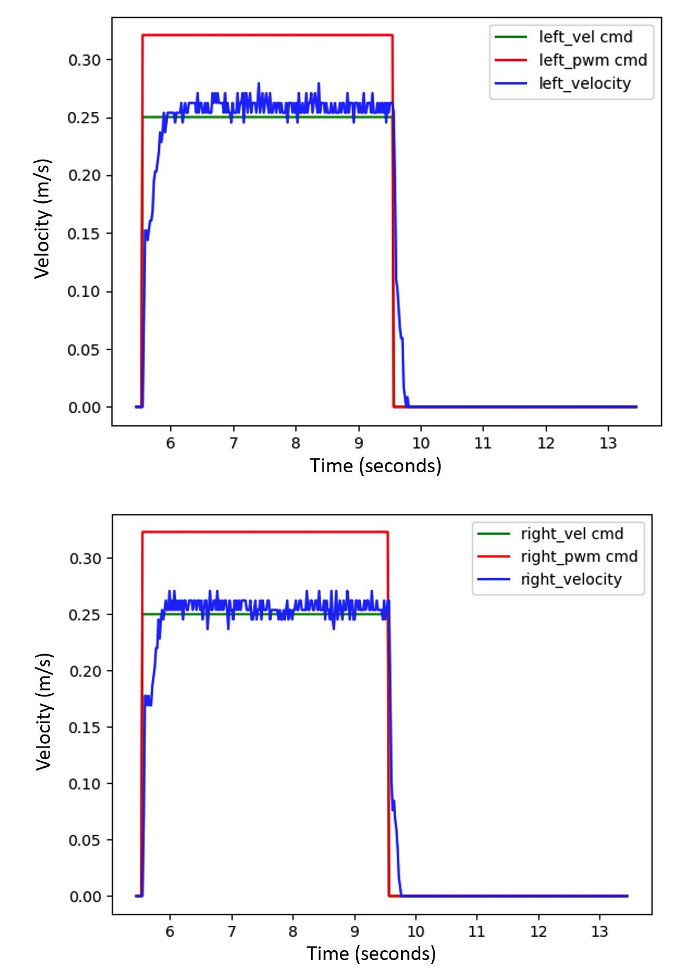
\includegraphics[width=0.84\linewidth]{image_1/figure_1_2_2.jpg}
\end{center}
   \caption{Results of controlling left and right wheels’ speeds with just feedforward control}
   \label{figure_1_2_2}
\end{figure}

In Figure \ref{figure_1_2_2}, the FF controller causes negative steady-state errors in the system. In order to minimize the steady-state error caused by the FF controllers, we used a unity gain (Kp=1) proportional FB controller. While the proportional controller helped minimize the steady-state error, it induced oscillations in the system’s response to step inputs. In order to damp out the oscillations, we added a derivative component to the FB controller. We experimented with the value of the gain associated with the derivative component (Kd) by steadily increasing it from 0.1 to its final value of 0.4. The results of running our robot with both FF and FB controllers are shown in Figure \ref{figure_1_2_3} below.


\begin{figure}[h]
\begin{center}
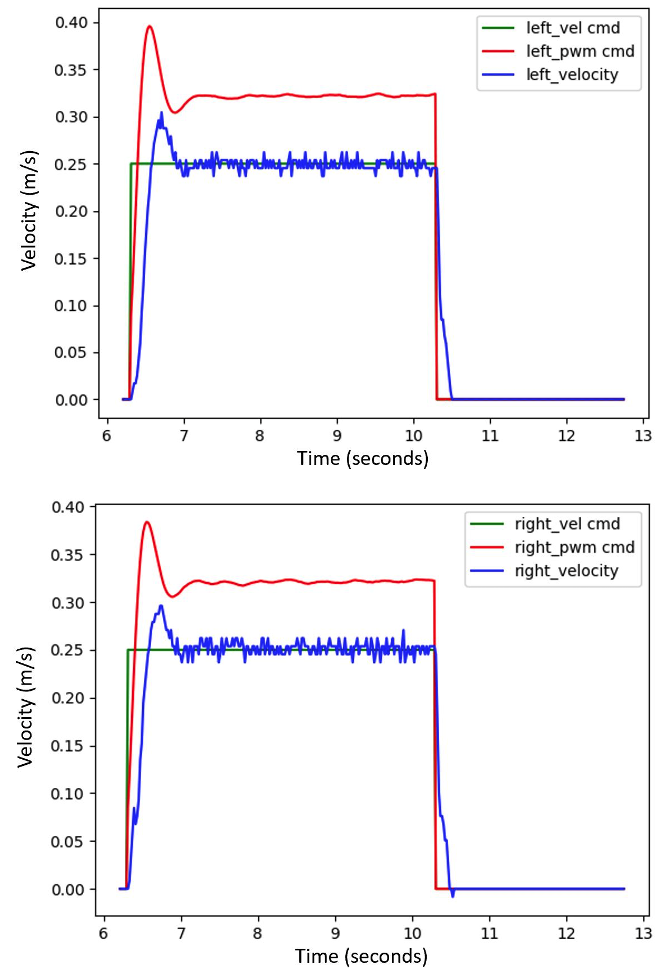
\includegraphics[width=0.81\linewidth]{image_1/figure_1_2_3.jpg}
\end{center}
   \caption{Controlling left/right wheels’ speeds with feedforward and feedback (PD) controllers}
	\label{figure_1_2_3}
\end{figure}


As can be seen in the graphs in Figure \ref{figure_1_2_3}, the FB controller minimizes the steady-state error caused by the FF controller. Figure \ref{Table_1_2_1} contains the parameters of the controllers described above. \\

\begin{figure}[h]
\begin{center}
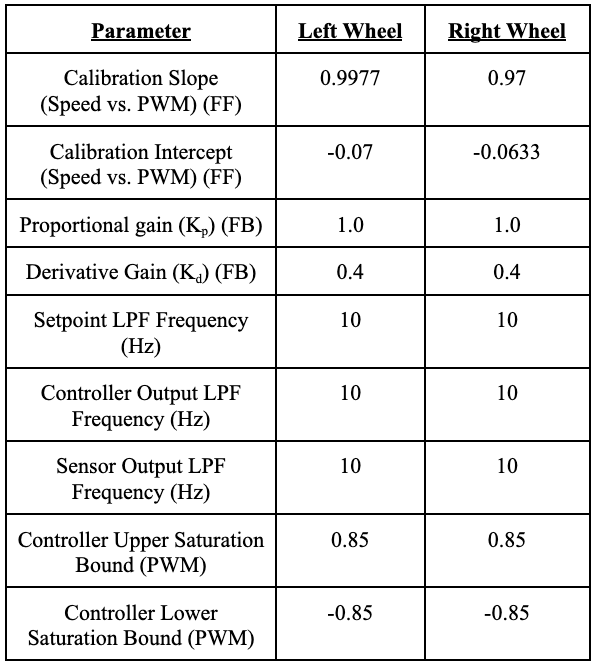
\includegraphics[width=0.82\linewidth]{image_1/Table_1_2_1.jpg}
\end{center}
    \caption{Controller parameters}
	\label{Table_1_2_1}
\end{figure}


\subsubsection{Odometry} \hfill\\

In order to validate our odometry model, we manually moved our robot by known distances and rotated it by known angles. We traversed our robot along a rectangle path (0.30 m x 0.25 m). A plot of the robot’s position estimate through odometry is shown in Figure \ref{figure_1_3}. On a clean, even surface, the robot’s pose estimate through odometry is extremely accurate and doesn’t warrant any correction parameters.\\

\begin{figure}[h]
\begin{center}
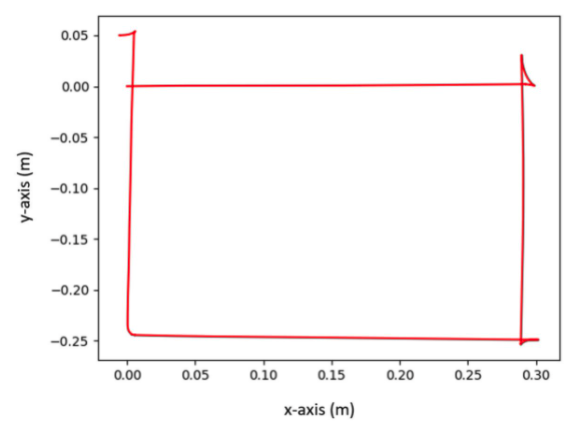
\includegraphics[width=0.9\linewidth]{image_1/figure_1_3.jpg}
\end{center}
   \caption{Odometry Validation}
   \label{figure_1_3}
\end{figure}



\subsubsection{Gyro Sensor Fusion}  \hfill\\

In order to perform odometry, we utilized the following equations,
$$\Delta s = \dfrac{\Delta sl+\Delta sr}{2}$$
where, $\Delta s$ is the displacement ($\Delta d$) of the center of the robot’s axle, $\Delta sl$ is the displacement of the left wheel of the robot, and $\Delta sr$ is the  displacement of the right wheel of the robot.
$$\alpha = \dfrac{\Delta sr -\Delta sl}{b}$$
where, $\alpha$ is the small change in the heading angle of the robot ($\Delta \theta, \Delta \theta_{odo}$) and b is the track width (distance between the left and right wheels) of the robot.

Finally, to ascertain how the position of our robot changes in the global/world frame,

$$\Delta x = \Delta d \times cos(\theta + \dfrac{\Delta \theta}{2})$$
$$\Delta y = \Delta d \times sin(\theta + \dfrac{\Delta \theta}{2})$$
where, $\Delta x$ and $\Delta y$ represent the changes in the x and y positions of the robot’s axle’s center in the global frame.\\

We obtained $\Delta sl$ and $\Delta sr$ by computing the difference between the current and previous encoder readings obtained from the encoders directly attached to the left and right motors respectively and by multiplying the obtained differences in encoder ticks by the constant converting it to meters.


Gyrodometry \cite{503813, borenstein1996measurement} is a method for combining measurements from a gyroscope with measurements from wheel encoders (odometry). The method based on the idea that non-systematic odometry error sources (such as bumps) impact the vehicle only during very short periods; typically a fraction of a second for each encounter. During these short instances the readings from the gyro and from odometry differ significantly. Such that in our implementation, if the wheels are not moving, we ignore the gyro reading. If gyro readings are significantly different than odometry, then we might hit a bump and should trust the gyro over odometry.

$$\Delta_{G-O}=\Delta\theta_{gyro}-\Delta\theta_{odo}$$
If $(|\Delta_{G-O,i}>\Delta\theta_{thres}|)$, which means the Gyro readings are significantly different than odometry, then
$$\theta_i=\theta_{i-1}+\Delta\theta_{gyro,i}$$
else,
$$\theta_i=\theta_{i-1}+\Delta\theta_{odo,i}$$

We obtained $\Delta \theta gyro$ by computing the difference between the current and previous readings of the Digital Motion Processed (DMP) Tait-Bryan angle (yaw) obtained from the Inertial Measurement Unit (IMU) on board the BeagleBone Blue (BBB). 

Here, by trial and error, we set the threshold to 6.25 degree, which is 0.109 in radian.\\


\subsubsection{Robot Frame Velocity Controller}  \hfill\\

For controlling the robot frame’s velocity, we used the following equations for relating the left and right wheels’ velocities with the robot forward and turning velocity commands
$$v_R=\omega(R+b/2)$$
$$v_L=\omega(R-b/2)$$
\noindent where, $v_R$ and $v_L$ are the velocities of right and left wheels respectively, $\omega$ is the angular/turning velocity of the robot, $R$ is the radius of the turning circle and $b$ is the track width. By using the relation between linear and angular velocities, the equations above can be rewritten as,
$$v_R=v+\omega b/2$$
$$v_L=v-\omega b/2$$
By breaking down the commanded robot frame forward and turning velocities into left and right wheel velocity commands, we utilized our closed-loop wheel speed controllers described in Section 1.2 to maneuver our robot with the desired forward and turning velocities. The parameters for the controller are listed in Figure \ref{Table_1_2_1}.


Plots of robot’s x-position (robot frame) vs. time for step inputs of varying magnitudes are shown in the Figures \ref{figure_1_5_1_1}, \ref{figure_1_5_1_2}, \ref{figure_1_5_1_3}.

\begin{figure}[h]
\begin{center}
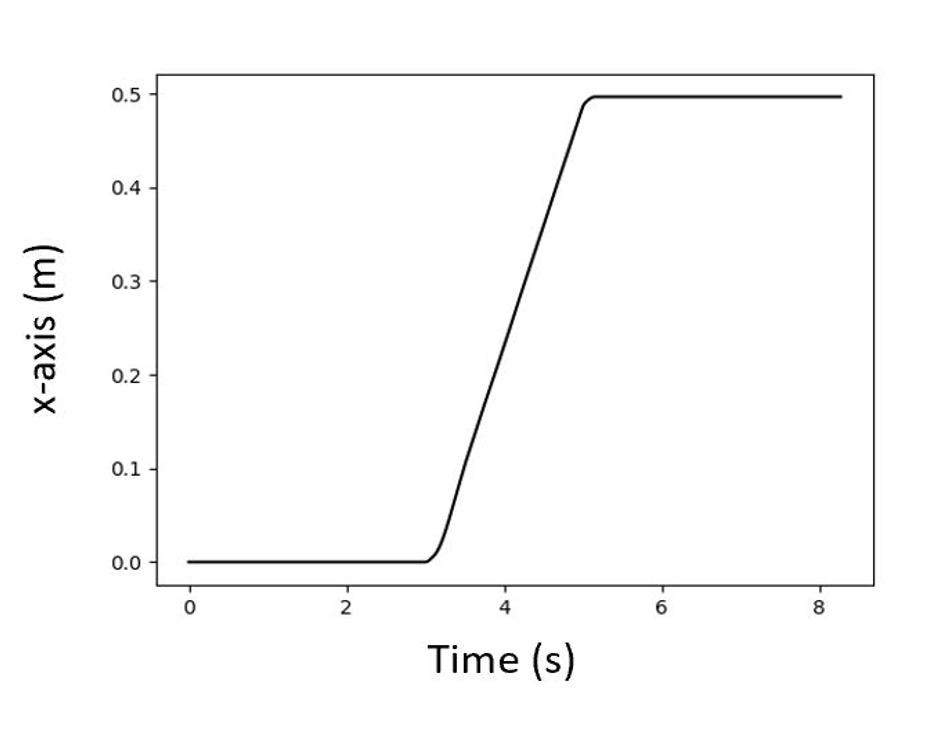
\includegraphics[width=0.8\linewidth]{image_1/figure_1_5_1_1.jpg}
\end{center}
   \caption{x position of 0.25 m/s for 2 s}
   \label{figure_1_5_1_1}
\end{figure}

\begin{figure}[h]
\begin{center}
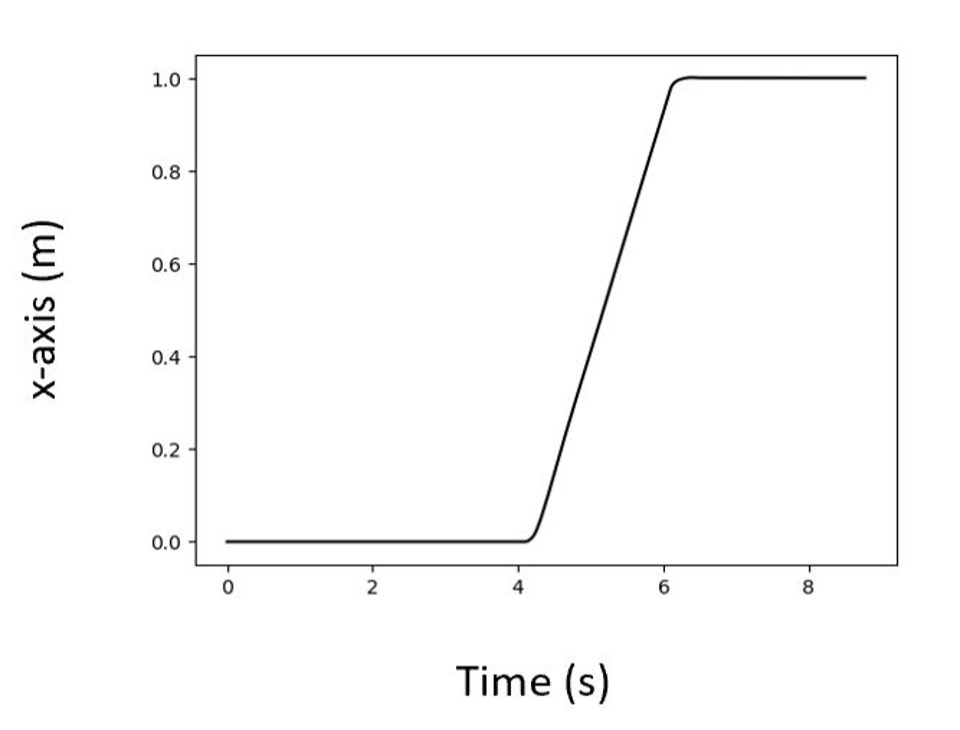
\includegraphics[width=0.8\linewidth]{image_1/figure_1_5_1_2.jpg}
\end{center}
   \caption{x position of 0.50 m/s for 2 s}
   \label{figure_1_5_1_2}
\end{figure}

\begin{figure}[H]
\begin{center}
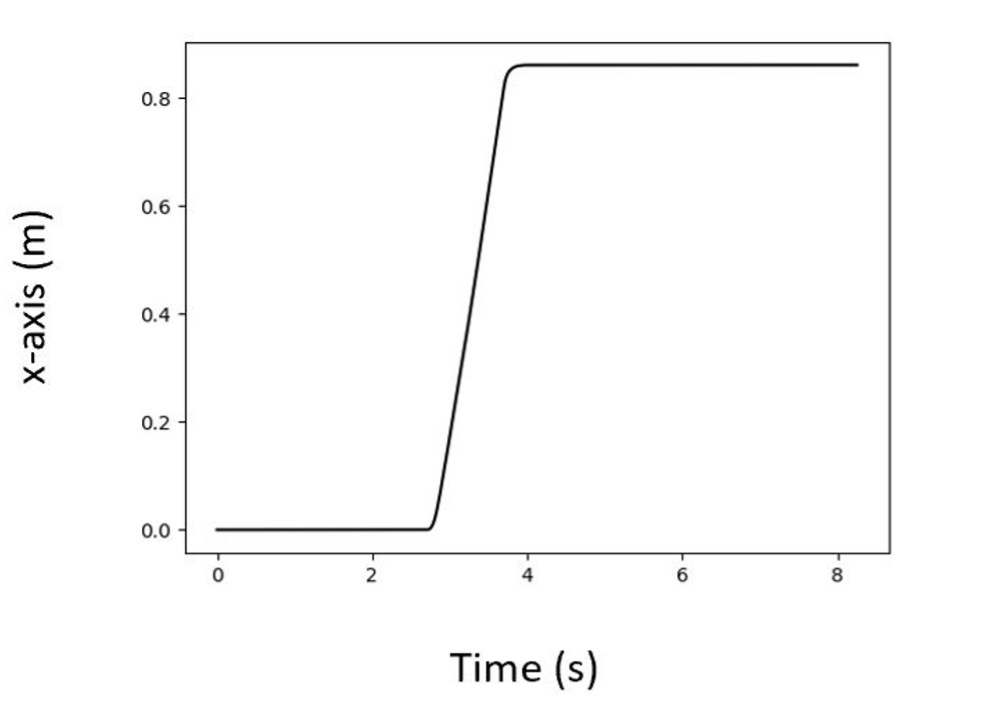
\includegraphics[width=0.8\linewidth]{image_1/figure_1_5_1_3.jpg}
\end{center}
   \caption{x position of 1.0 m/s for 1 s}
   \label{figure_1_5_1_3}
\end{figure}


From the plots of x position vs. time above, we can see that the controller works well for 0.25 m/s and 0.50 m/s step commands, however, it doesn’t work well for a step input of 1.0 m/s. In order to move at 1m/s, the motors need very high duty cycles ($>$90\%) very quickly. As a result, the robot often skids and becomes difficult to control. Furthermore, under full load conditions, the robot never reaches a speed of 1.0 m/s even with a 100\% duty cycle input.

Plots of robot’s heading (robot frame) vs. time for step inputs of varying magnitudes are shown in the Figures \ref{figure_1_5_2_1}, \ref{figure_1_5_2_2}, \ref{figure_1_5_2_3} below.

\begin{figure}[h]
\begin{center}
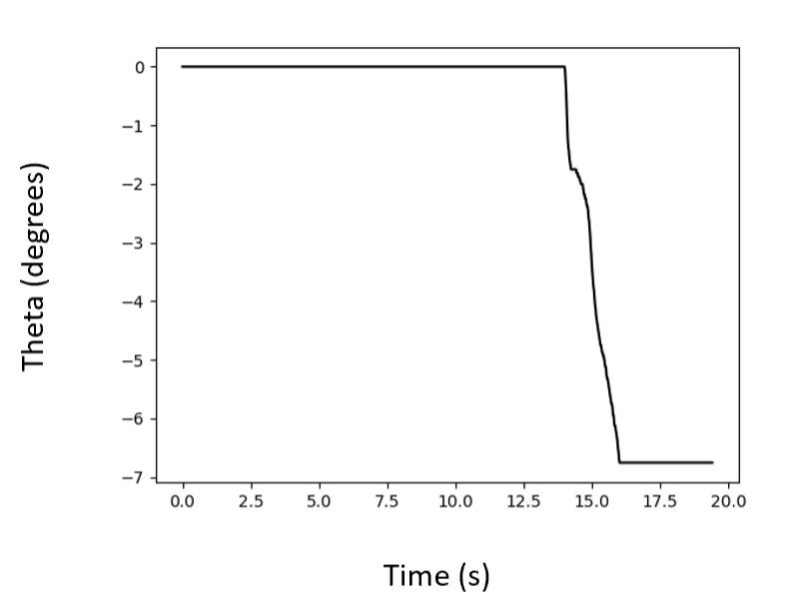
\includegraphics[width=0.77\linewidth]{image_1/figure_1_5_2_1.jpg}
\end{center}
   \caption{heading angle of $\pi$/8 rad/s for 2s}
   \label{figure_1_5_2_1}
\end{figure}

\begin{figure} [h]
\begin{center}
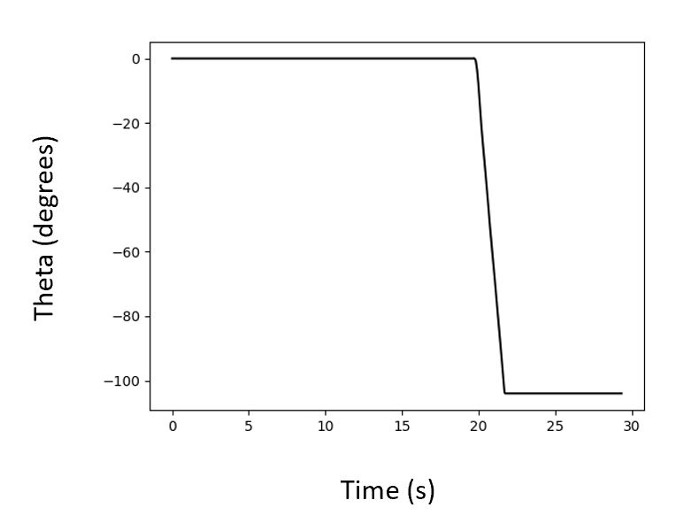
\includegraphics[width=0.77\linewidth]{image_1/figure_1_5_2_2.jpg}
\end{center}
   \caption{heading angle of $\pi$/2 rad/s for 2s}
   \label{figure_1_5_2_2}
\end{figure}

\begin{figure} [h]
\begin{center}
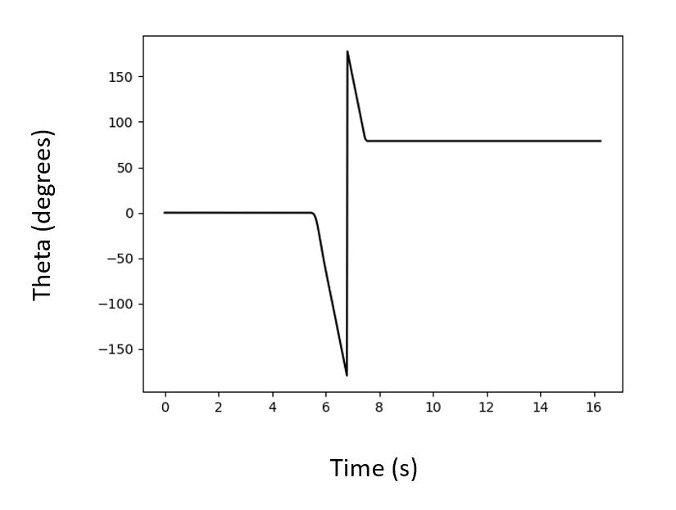
\includegraphics[width=0.77\linewidth]{image_1/figure_1_5_2_3.jpg}
\end{center}
   \caption{heading angle of $\pi$ rad/s for 2s}
   \label{figure_1_5_2_3}
\end{figure}

\newpage
The plot shown in Figure \ref{figure_1_5_2_3} shows a sudden change in the value of the heading angle. The reason for the sudden change is that the heading angle of the robot is always wrapped between $[-\pi, \pi]$ radians. Therefore, the angle goes back to $\pi$ when it exceeds $-\pi$ while rotating from the clockwise (CW) direction and goes to $-\pi$ when it exceeds $\pi$ while rotating from the counter-clockwise (CCW) direction.\\

\subsubsection{Motion Controller} \hfill\\

For the motion controller, we used a Rotate-Translate-Rotate (RTR) \cite{journals/ker/Parsons04f,spong2005robot} type controller to track waypoints. Specifically, our controller consists of two elements. One, a turn maneuver and two, a straight maneuver. The turn maneuver causes the robot to rotate such that it points (heads) in the direction of the target pose. It does so by controlling the rotation of the robot at its current position such that at steady state, the robot points towards the target. Since we do not care about the heading angle of our robot at its target location, we did not incorporate an element responsible for ensuring that the robot heads in a specific direction upon reaching the target position in our controller. Therefore, in essence, our controller works like a RTR controller for the first n-1 points in our trajectories consisting of n total points where n is a positive integer greater than 1.

The turn maneuver is realized by the mathematical equations shown below:
$$\omega_{sp}=K_\omega \alpha$$
$$v_{sp}=0$$
where, $\omega_{sp}$ is the turn velocity (angular velocity), $v_{sp}$ the translational velocity of our robot, and $K_\omega$ is the proportional gain associated with the required turning angle, $\alpha$ (angle between current heading and heading towards goal).

For the straight maneuver, we used both the translational and turning velocity components. Using both components, ensures that we move along a straight line and maintain by dynamically correcting our direction of motion in case of any deviations. Using only translational velocity in the straight maneuver can cause the robot to deviate from its intended path because of a multitude of reasons. Difference in the transient response of each wheel, difference in the settling time of each wheel, difference in the friction associated with the patch of ground each wheel is rotating on, and the like. Mathematical equations utilized for implementing the straight maneuver component of our controller are as follows:

$$\omega_{sp}=K_\omega \alpha$$
$$v_{sp}=K_d d$$
where,  $\omega_{sp}$, $K_\omega$, and $\alpha$ are the same as above. $v_{sp}$  is now directly proportional to the amount of distance the robot needs to traverse, d and the constant of proportionality is the proportional gain, $K_d$. The parameters and thresholds are shown in table below. d\_threshold and $\alpha$\_threshold are the thresholds that serve as error tolerances about the target poses.\\

\begin{center}
\begin{tabular}{ |c|c| } 
 \hline
 \textbf{Parameters} & \textbf{Values} \\ 
 \hline
 $K_\omega$ & 0.8 \\ 
 \hline
 $K_d$ & 0.5 \\ 
 \hline
 d\_threshold (m) & 0.05 \\
 \hline
 $\alpha$\_threshold (radians)& 0.07 \\
 \hline
\end{tabular}
\end{center}

The plot of dead reckoning estimated pose of our robot by commanding it to drive a 1m square four times is shown below.
\begin{figure}[h]
\begin{center}
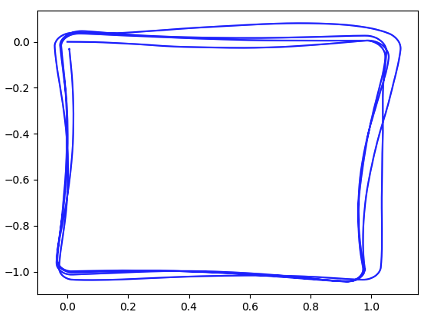
\includegraphics[width=0.8\linewidth]{image_1/figure_1_6_1.jpg}
\end{center}
   \caption{Dead reckoning position estimation by driving a 1m square four times}
   \label{figure_1_6_1}
\end{figure}

The plots of the robots linear and rotational velocity as it drives one loop around the square are shown below.

\begin{figure}[h]
\begin{center}
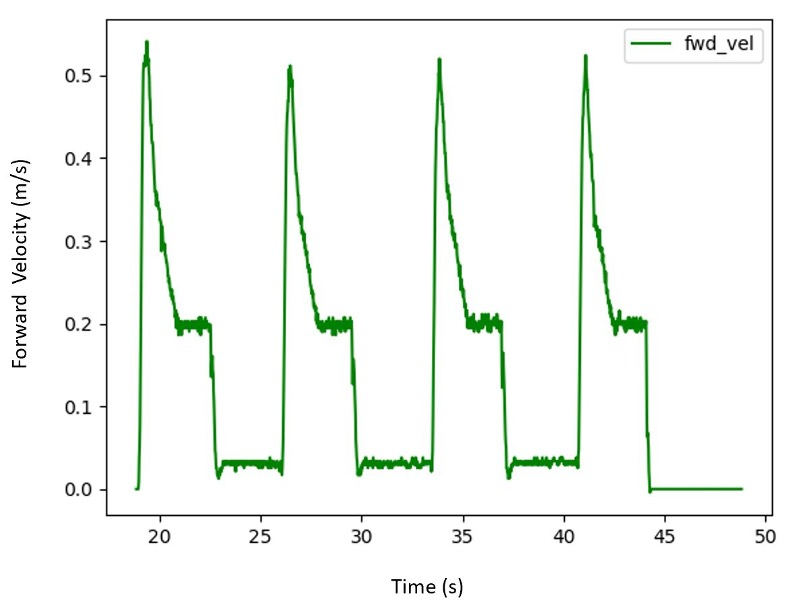
\includegraphics[width=1\linewidth]{image_1/figure_1_6_2_linear.jpg}
\end{center}
   \caption{Forward velocity of the robot as a function of time as it drives a square path once}
   \label{figure_1_6_2_linear}
\end{figure}

\begin{figure}[h]
\begin{center}
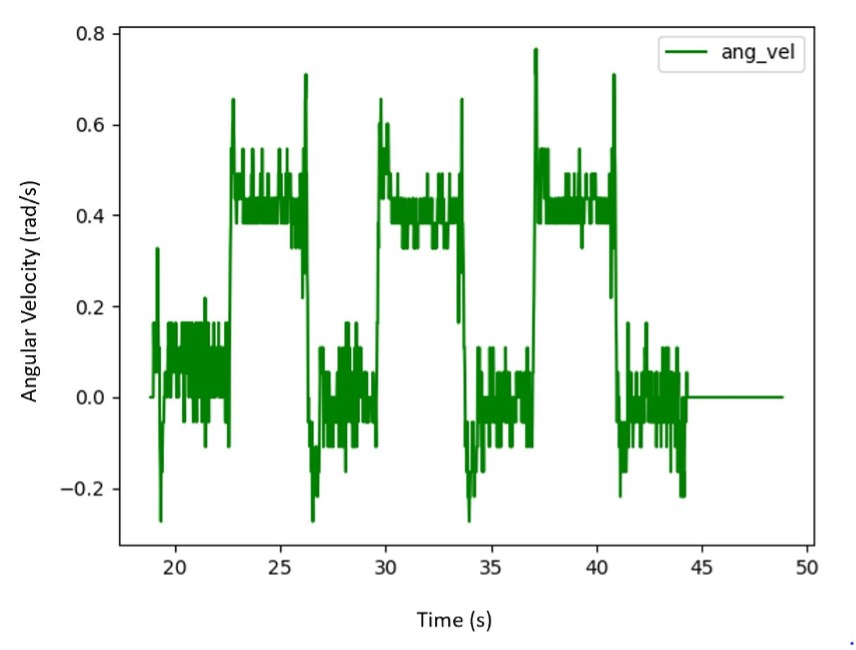
\includegraphics[width=1\linewidth]{image_1/figure_1_6_2_angular.jpg}
\end{center}
   \caption{Angular velocity of the robot as a function of time as it drives a square path once}
   \label{figure_1_6_2_angular}
\end{figure}


\newpage
\subsection{Simultaneous Localization and Mapping (SLAM)} 

\subsubsection{Mapping} \hfill\\

Figure 16 shown below depicts a map/obstacle distance grid for a provided .log file.

\begin{figure}[h]
\begin{center}
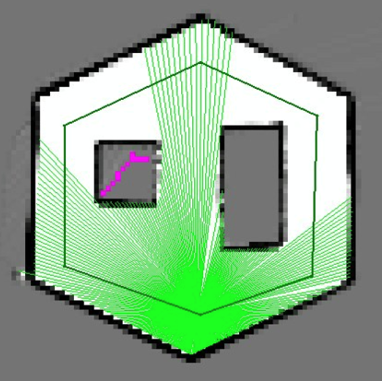
\includegraphics[width=0.6\linewidth]{image_2/figure_2_1.jpg}
\end{center}
   \caption{Map from the log file obstacle slam 10mx10m 5cm}
   \label{figure_2_1}
\end{figure}

\subsubsection{Monte Carlo Localization}\hfill\\

\paragraph{Action Model}  \hfill\\

From odometry, we have previous and current poses, which we can use to calculate the changes in translation and rotation.

\begin{figure}[h]
\begin{center}
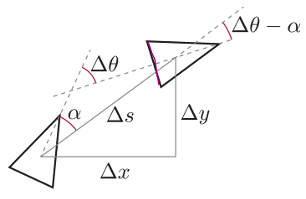
\includegraphics[width=0.5\linewidth]{image_2/figure_2_2_1.jpg}
\end{center}
   \caption{Action model}
   \label{figure_2_2_1}
\end{figure}

$$\Delta s^2 = \Delta x^2 + \Delta y^2$$
$$\alpha=atan2(\Delta y, \Delta x)-\theta_{t-1}$$
Thus, we modelled action as rotation, translation, and rotation (RTR): $u=[\alpha \; \; \Delta s \; \; \Delta \theta - \alpha]$. Figure 17 below depicts the RTR model used above. 

Following that, we further model the action error:
\begin{itemize}
  \item Turn$(\alpha + \varepsilon_1)$
  \item Travel$(\Delta s + \varepsilon_2)$
  \item Turn$(\Delta \theta -\alpha + \varepsilon_3)$
\end{itemize}

Using the above equations, we assigned Gaussian error $\varepsilon$ to both translational motion and rotational motion. Since we calibrated odometry to eliminate systematic errors, we have a 0 mean error Gaussian distribution. As a consequence, we assume that there is no systematic error.

Then we use following equations to combine the error and changes together to update the new position.
Given $u=[\alpha \; \; \Delta s \; \; \Delta \theta - \alpha]$:

\begin{gather*}
 \begin{bmatrix} x_t \\ y_t \\ \theta_t \end{bmatrix}
 =
 \begin{bmatrix} x_{t-1} \\ y_{t-1} \\ \theta_{t-1} \end{bmatrix}
 =
  \begin{bmatrix}
   (\Delta s + \varepsilon_2)cos(\theta_{t-1}+\alpha + \varepsilon_1)\\
   (\Delta s + \varepsilon_2)sin(\theta_{t-1}+\alpha + \varepsilon_1)\\
   \Delta \theta + \varepsilon_1 + \varepsilon_3 
   \end{bmatrix}
\end{gather*}

where:
\begin{itemize}
  \item $\varepsilon_1 \sim \mathcal{N} (0, k_1 |\alpha|)$
  \item $\varepsilon_2 \sim \mathcal{N} (0, k_2 |\Delta s|)$
  \item $\varepsilon_3 \sim \mathcal{N} (0, k_1 |\Delta \theta - \alpha|)$
\end{itemize}

To tune the action model \cite{pbr}, we performed straight line experiments and rotation experiments to determine reasonable values of $k_1$ and $k_2$.
\begin{itemize}
  \item If both $k_1$ and $k_2$ are too small: it will track odometry position only, and take it as the true pose.
  \item If the dispersion is too large, particles will be everywhere.
\end{itemize}
By trial and error, we chose these two numbers because they worked well.

\begin{center}
\begin{tabular}{ |c|c| } 
 \hline
 \textbf{Parameters} & \textbf{Values} \\ 
 \hline
 $k_1$ & 0.01 \\ 
 \hline
 $k_1$ & 0.01 \\ 
 \hline
\end{tabular}
\end{center} 


\paragraph{Sensor Model and Particle Filter}  \hfill\\

Time taken to update the particle filter for 100, 300, 500 and 1000 particles is tabulated in Table below.
\begin{center}
\begin{tabular}{ |c|c| } 
 \hline
 \textbf{Particle Numbers} & \textbf{Time (microseconds)} \\ 
 \hline
 100 & 4573.53 \\ 
 \hline
 300 & 11786 \\ 
 \hline
 500 & 17683.5 \\ 
 \hline
 1000 & 31228.3 \\ 
 \hline
\end{tabular}
\end{center} 



10Hz can be converted to 0.1 second (period) which is 100,000 microseconds. From the table above, we know that 1000 particles take 31228.3 microseconds to update, the estimated maximum number of particles can be supported at 10Hz is 3200. 300 particles at the midpoint of each 1m translation for a square and at the corners after having turned 90 degrees can be seen in Figure 18 below.\\
\begin{figure}[h]
\begin{center}
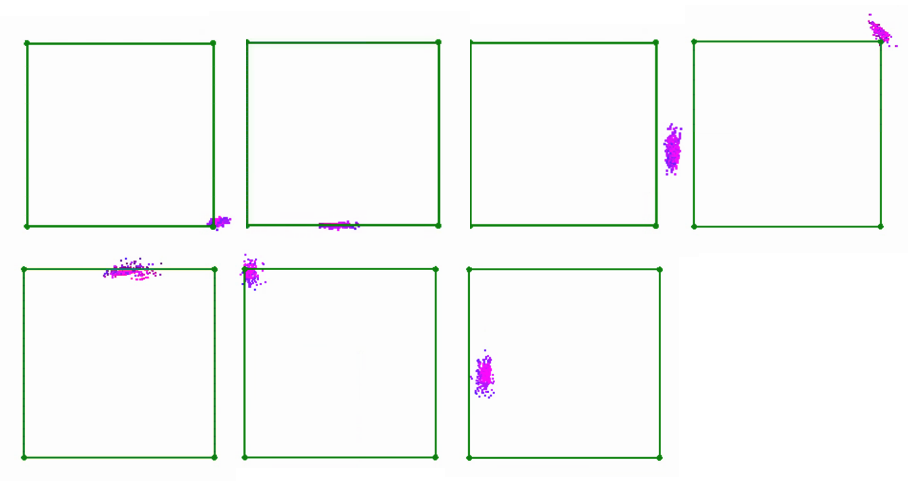
\includegraphics[width=1\linewidth]{image_2/figure_2_2_2.jpg}
\end{center}
   \caption{300 particles at the midpoint of each 1m translation and at the corners after having turned 90°}
   \label{figure_2_2_2}
\end{figure}

Plot showing how the pose error difference between the SLAM and Odometry poses evolves over time is shown in Figure 19 below.

\begin{figure}[h]
\begin{center}
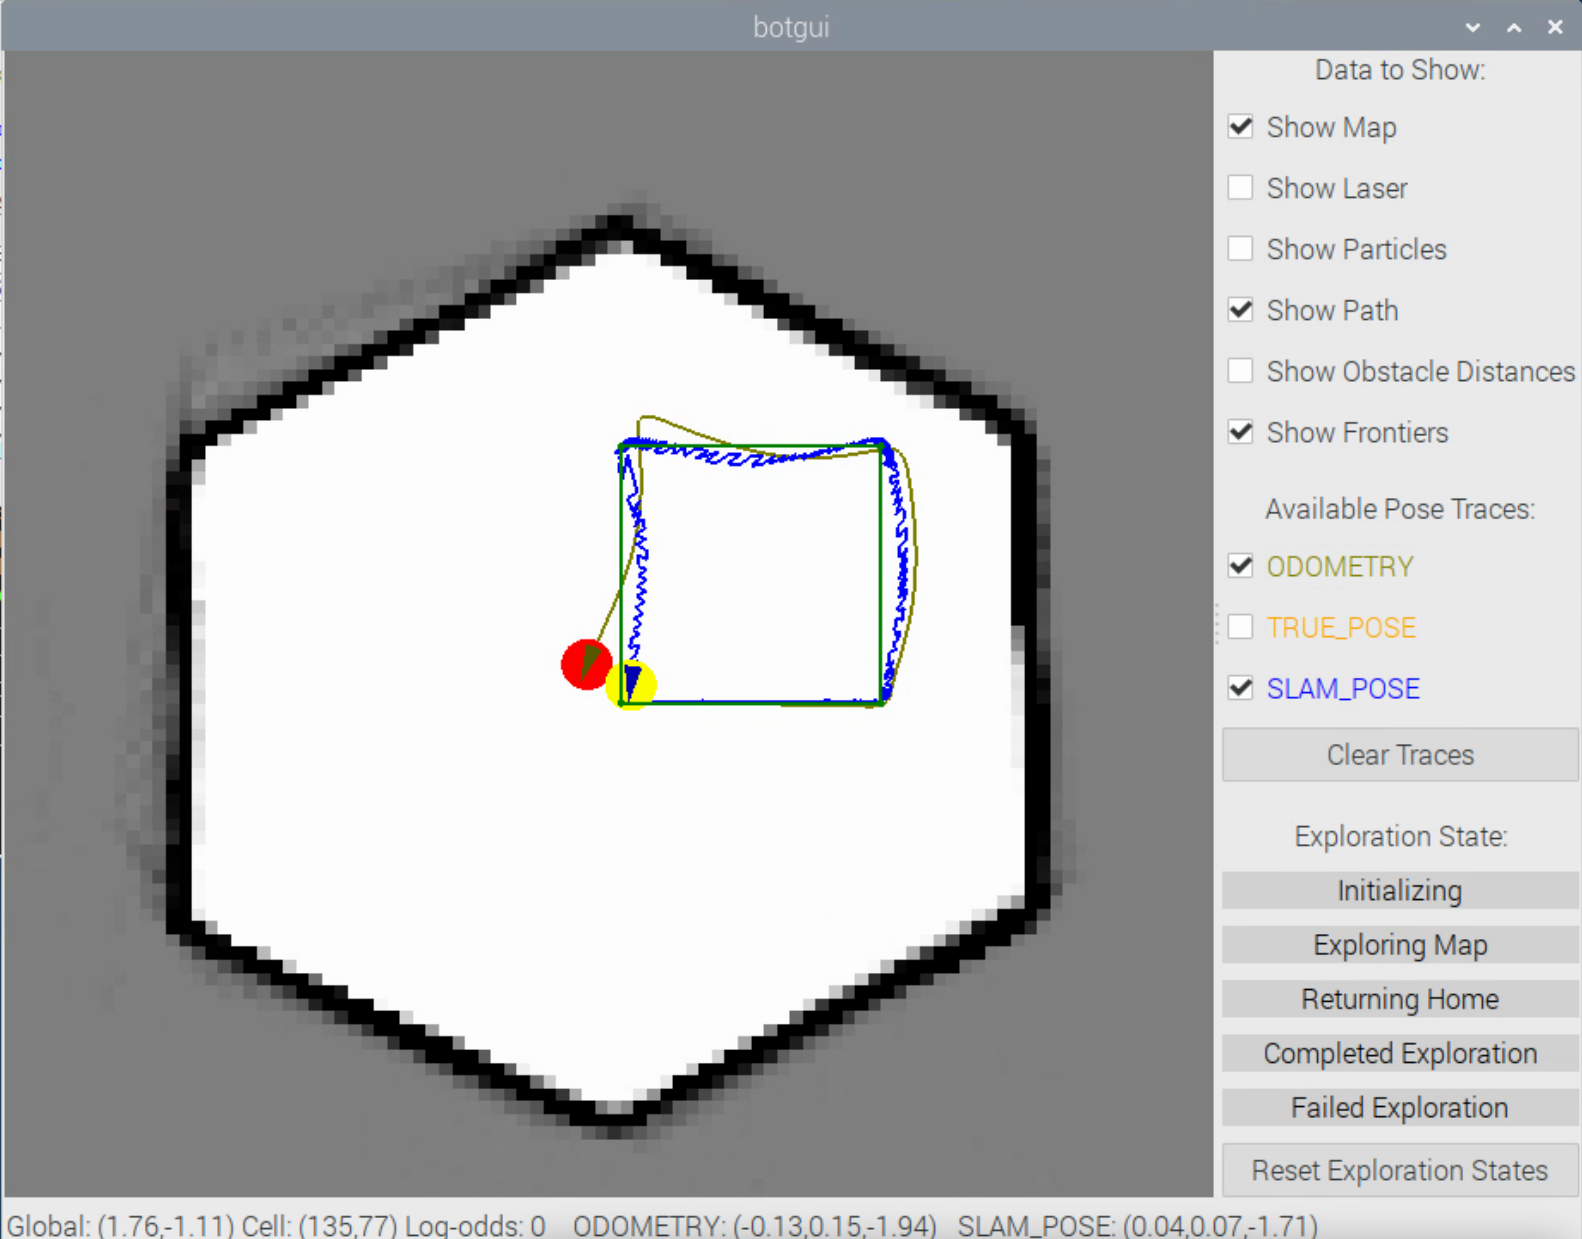
\includegraphics[width=1\linewidth]{image_2/figure_2_2_2_4.jpg}
\end{center}
   \caption{pose error difference between the SLAM and Odometry poses}
   \label{figure_2_2_2_4}
\end{figure}


\subsubsection{Combined Implementation}  \hfill\\

A block diagram showing how the SLAM system components interact is shown in Figure 20 below.\\

\begin{figure}[h]
\begin{center}
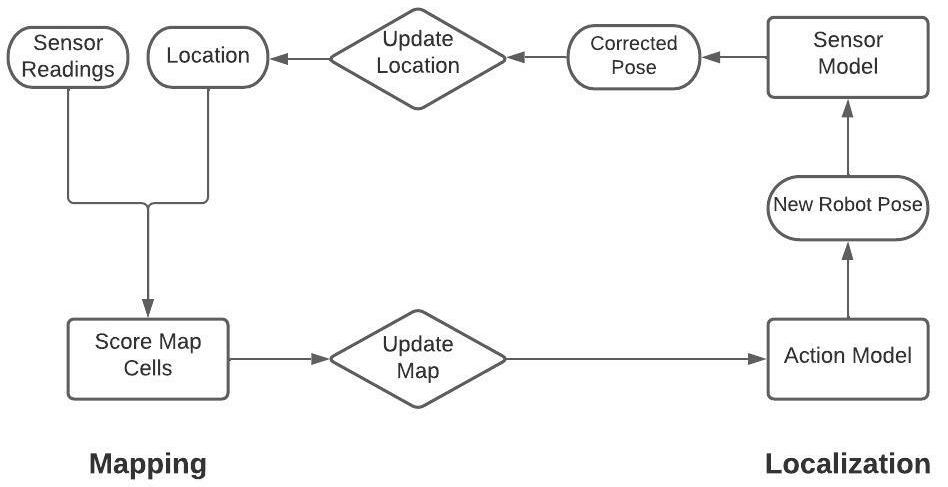
\includegraphics[width=1\linewidth]{image_2/figure_2_3_1.jpg}
\end{center}
   \caption{SLAM system}
   \label{figure_2_3_1}
\end{figure}
\newpage
We compared the estimated poses from our SLAM system against the ground-truth poses in obstacle\_slam\_10mx10m\_5cm.log and obtained the RMS errors tabulated in the table below.

\begin{center}
\begin{tabular}{ |c|c| } 
 \hline
 \textbf{RMS} & \textbf{Values} \\ 
 \hline
 Distance & 0.07739 \\ 
 \hline
 x & 0.05560 \\ 
 \hline
 y & 0.05382 \\
 \hline
 theta & 0.07467 \\
 \hline
\end{tabular}
\end{center}


\subsection{Planning and Exploration}

\subsubsection{Path Planning} \hfill\\

Figure \ref{figure_3_2} shown below depicts a path planned by our A* path planning algorithm in a maze environment with the actual path driven of our robot overlayed on top.

\begin{figure}[h]
\begin{center}
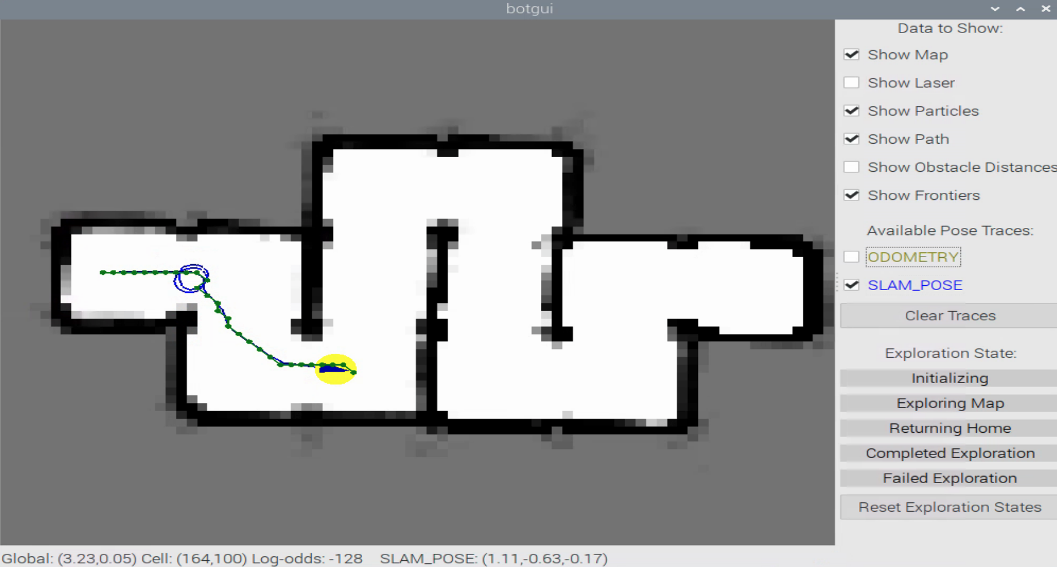
\includegraphics[width=1\linewidth]{image_3/figure_3_2.jpg}
\end{center}
   \caption{Path planned through our A* algorithm and actual path traversed by our robot in a maze environment}
   \label{figure_3_2}
\end{figure}

Statistics on our path planning execution times for each of the example problems in the data/astar folder are shown in the Table below.

\begin{center}
\resizebox{\columnwidth}{!}{
\begin{tabular}{ |c|c|c|c|c|c| } 
 \hline
 ($\mu s$) &Min & Mean & Max & Median & std dev\\ 
 \hline
 convex\_grid & 996 & 996 & 996 & 0 & 0 \\ 
 \hline
 empty\_grid & 3464 & 7559.33 & 10127 & 10127 & 2926.8 \\ 
 \hline
 maze\_grid &  881 & 6554.75 & 11261 & 5109 & 3945.07 \\ 
 \hline
 narrow\_grid &  5787 & 567350 & 996 & 1.12891e6 & 0 \\ 
 \hline
 wide\_grid & 10562&  923133 & 1.72044e6 & 1.72044e6 &  702798 \\ 
 \hline
\end{tabular}}
\end{center} 

\begin{center}
\resizebox{\columnwidth}{!}{
\begin{tabular}{ |c|c|c|c|c|c| } 
 \hline
 ($\mu s$) &Min & Mean & Max & Median & std dev\\ 
 \hline
 convex\_grid & 40 & 112 & 161 & 135 & 52.0064 \\ 
 \hline
 empty\_grid & 38 & 90 & 142 & 0 & 52 \\ 
 \hline
 filled\_grid &  39 & 62.4 & 89 & 63 & 19.7342\\ 
 \hline
 narrow\_grid &  90 & 642961 & 1.92866e6 & 134 & 909126 \\ 
 \hline
 wide\_grid & 61&  61& 61& 0&  0\\ 
 \hline
\end{tabular}}
\end{center} 

From the statistics above, we can conclude that our path planning algorithm (A*) is optimal and fast.\\


\subsubsection{Exploration} \hfill\\

Using connected components search in the occupancy grid we found the frontiers. A 4-way search was carried around each free space cell to locate the frontier cells. Upon locating the frontier cells, an 8-way search grew the frontier. All the frontiers were identified using the \textit{find\_map\_frontiers()} function.\\

Once we had a collection of frontiers, we chose which frontier to explore. Among the available frontiers, we calculated the Euclidean distance from the current pose to the start cell of each available frontier. The one with the shortest distance was returned and a path to it was planned using our A-star algorithm. Once there are no frontiers left to explore, the program ensures that all free space is surrounded by occupied cells.\\

\subsubsection{Map Localization with Unknown Starting Position}  \hfill\\
\indent Particles were uniformly distributed using a uniform distribution function. The distance of each particle from the nearest frontier was calculated. The pose with the farthest distance from the frontier was chosen and the mobilebot moved along the direction towards that frontier. The pose was updated, and particles were redistributed. The same procedure was iterated until a narrow distribution was obtained.\\


\ifCLASSOPTIONcaptionsoff
  \newpage
\fi

% Include your citations in the references.bib file
\nocite{*}
\bibliographystyle{IEEEtran}
\bibliography{references.bib}
\end{document}